\documentclass{article}
\usepackage{graphicx}
\usepackage{float} % To use figures with H option
\usepackage{hyperref} % For adding hyperlinks

\title{React Native Development Environment Setup and Todo List Application}
\author{Jeevan Tubinakere Govindaraju}
\date{November 18, 2024}

\begin{document}

\maketitle

\begin{center}
\href{https://github.com/Jeevan-369/Lab3}{GitHub Repository: https://github.com/Jeevan-369/Lab3}
\end{center}

\section{Introduction to React Native}
React Native is an open-source framework developed by Facebook that allows developers to create mobile applications using JavaScript and React. Its primary advantage is the ability to develop apps for both iOS and Android platforms from a single codebase, significantly reducing development time and effort. This means you can write your application once and deploy it on both platforms, taking advantage of native performance and user experience.

\subsection{Key Features of React Native}
\begin{itemize}
    \item \textbf{Cross-Platform Compatibility:} Build applications that run seamlessly on both iOS and Android.
    \item \textbf{Hot Reloading:} Instantly see the results of changes made to your code, speeding up the development process.
    \item \textbf{Rich Ecosystem:} Access a wide range of libraries and components, making it easier to add complex functionalities.
\end{itemize}

% After your introduction section but before the subsections

\noindent\textbf{\Large Task 1: Set Up the Development Environment (50 Points)}\\[0.5cm]
\noindent In this task, I set up the development environment to build React Native applications.\\[1cm]

\subsection{Step 1: Install Node.js and Watchman}
To complete this step:
\begin{enumerate}
    \item Installed Node.js from the \href{https://nodejs.org/en}{official website}, which also included npm.
    \item Installed Watchman (optional) using Homebrew on macOS:
    \begin{verbatim}
    brew install watchman
    \end{verbatim}
\end{enumerate}

\subsection{Step 2: Install React Native CLI}
Installed the React Native CLI using:
\begin{verbatim}
    npm install -g react-native-cli
\end{verbatim}
Alternatively, used npx:
\begin{verbatim}
    npx react-native init YourProjectName
\end{verbatim}

\subsection{Step 3: Set Up Android Studio (or Xcode for iOS)}
For Android:
\begin{enumerate}
    \item Installed Android Studio and enabled SDK tools including Android SDK Build-Tools, Platform-Tools, Emulator, and Google Play Services.
    \item The setup was verified as shown in Figure~\ref{fig:sdk_setup}.
\end{enumerate}
For iOS:
\begin{itemize}
    \item Installed Xcode and command line tools using:
    \begin{verbatim}
    xcode-select --install
    \end{verbatim}
\end{itemize}

\begin{figure}[H]
    \centering
    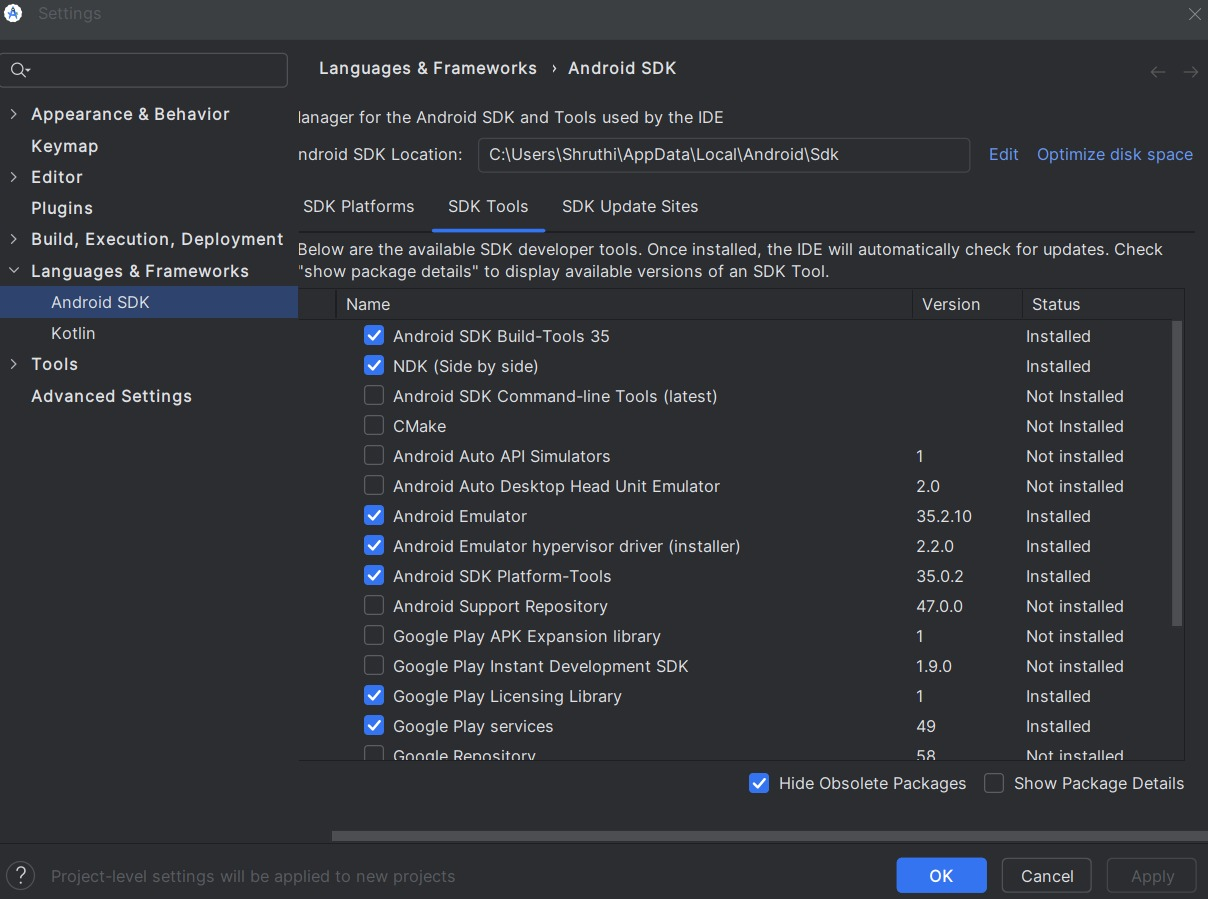
\includegraphics[width=0.7\textwidth]{SDK setup.jpeg}
    \caption{Android SDK Setup in Android Studio}
    \label{fig:sdk_setup}
\end{figure}

\subsection{Step 4: Create a New React Native Project}
Initialized a new project using:
\begin{verbatim}
    npx react-native init YourProjectName
    cd YourProjectName
\end{verbatim}

\subsection{Step 5: Open the Project in Visual Studio Code}
Opened the folder in VS Code and installed the React Native Tools extension.

\subsection{Step 6: Start the Metro Bundler}
Started the Metro Bundler using:
\begin{verbatim}
    npx react-native start
\end{verbatim}

\begin{figure}[H]
    \centering
    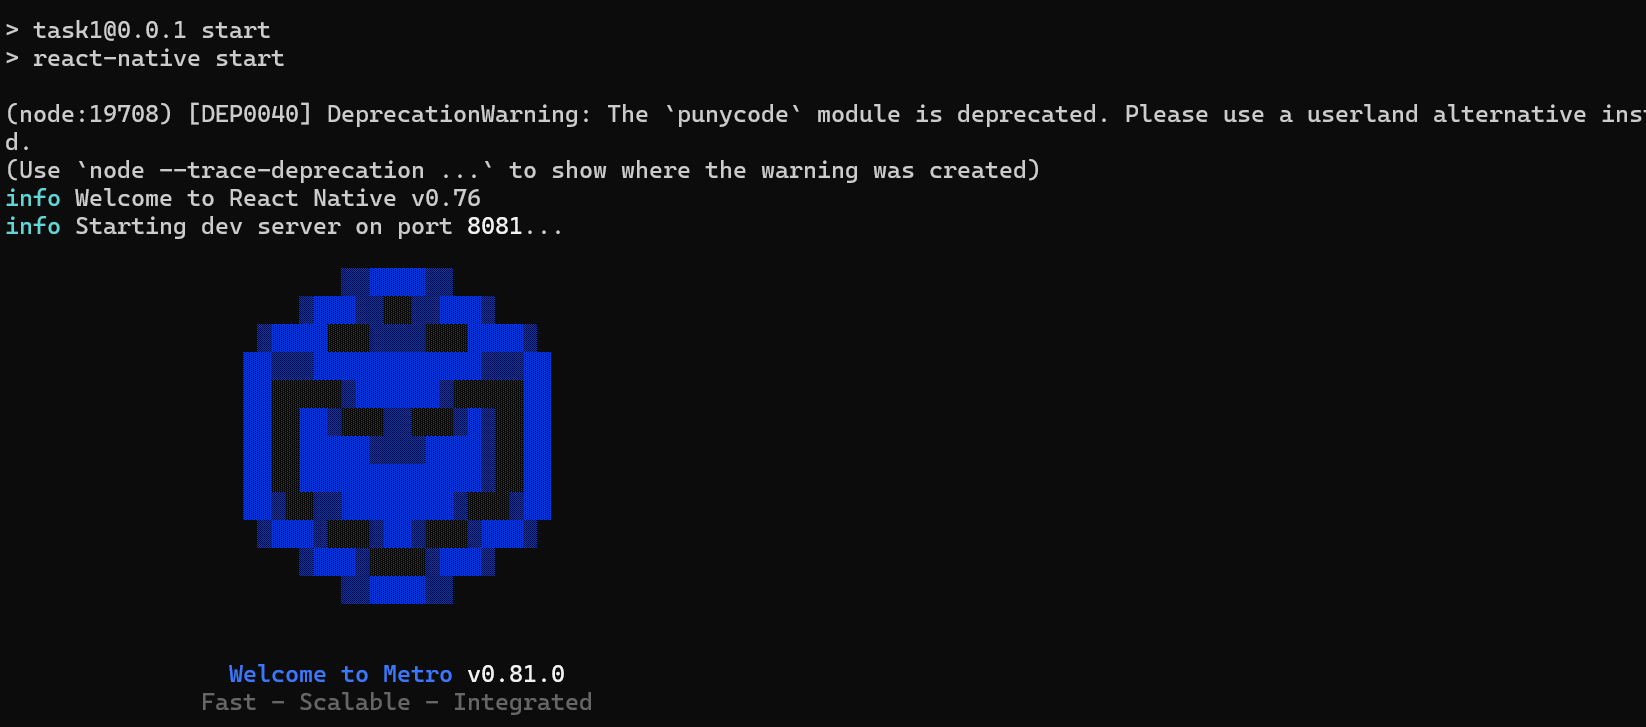
\includegraphics[width=0.7\textwidth]{start metro bumdler.png}
    \caption{Metro Bundler Started in Terminal}
    \label{fig:metro_bundler}
\end{figure}

\subsection{Step 7: Run the App on Emulator or Device}
For Android:
\begin{verbatim}
    npx react-native run-android
\end{verbatim}
For iOS:
\begin{verbatim}
    npx react-native run-ios
\end{verbatim}

\begin{figure}[H]
    \centering
    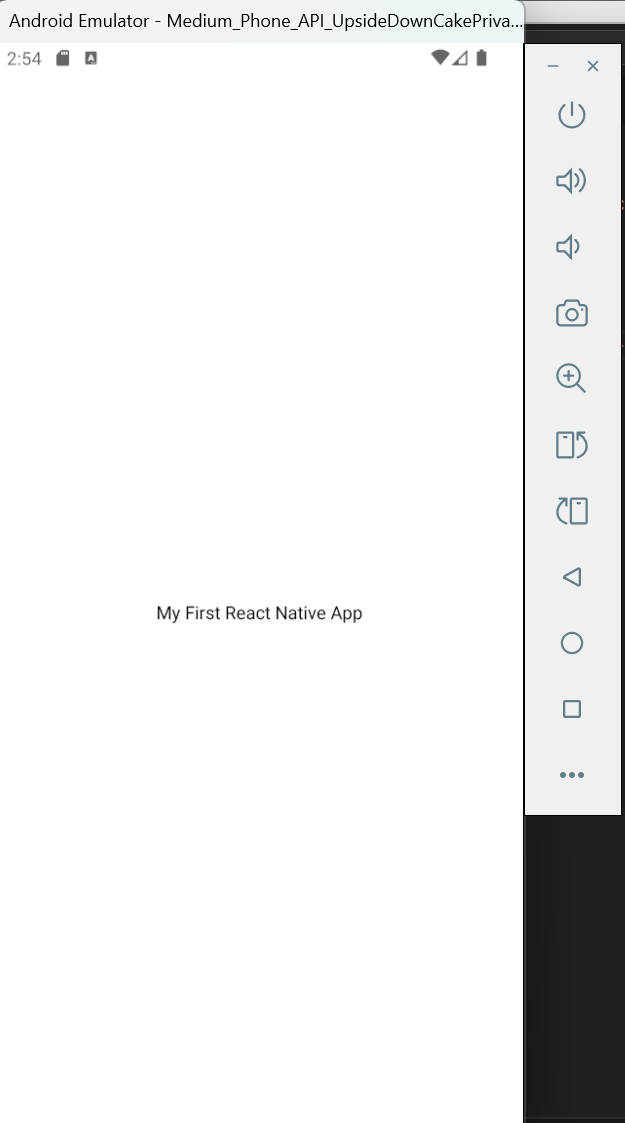
\includegraphics[width=0.5\textwidth]{app on emulator.png}
    \caption{App running on Android Emulator}
    \label{fig:emulator}
\end{figure}

\subsection{Step 8: Run the App Using Expo}
Installed and created a new Expo project:
\begin{verbatim}
    npm install -g expo-cli
    npx expo init YourProjectName
    npx expo start
\end{verbatim}
Connected a physical device using the Expo Go app.

\begin{figure}[H]
    \centering
    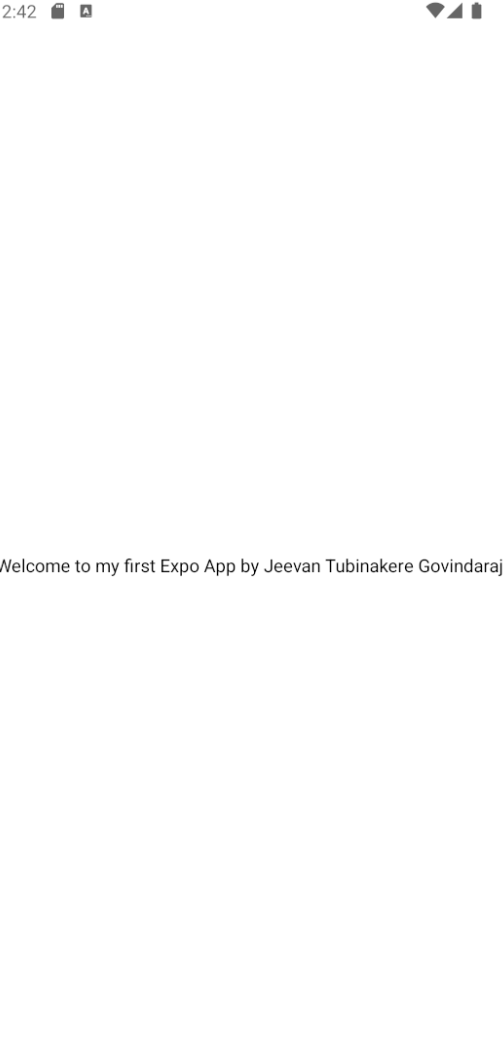
\includegraphics[width=0.5\textwidth]{app on physical device.png}
    \caption{App running on Physical Device using Expo}
    \label{fig:expo_device}
\end{figure}

\subsection{Submission Requirements for Task 1}
\begin{itemize}
    \item \textbf{Screenshots}: 
    \begin{itemize}
        \item Figure~\ref{fig:emulator} shows the app running on the Android emulator.
        \item Figure~\ref{fig:expo_device} shows the app running on a physical device using Expo.
        \item Figure~\ref{fig:metro_bundler} shows the Metro Bundler running in the terminal.
    \end{itemize}
    \item \textbf{Setting Up an Emulator}: Steps to set up the emulator are explained in Section~\ref{fig:sdk_setup}. Challenges faced included issues that sometimes, the emulator might fail to start due to insufficient hardware acceleration. Ensure that virtualization support is enabled in the BIOS.
    \item \textbf{Running on a Physical Device Using Expo}: The process for running the app on a physical device is explained in Step 8, Challenges faced included issues with Ensuring your phone and development machine are on the same Wi-Fi network. If you encounter issues, restarting the Expo server (expo start -c) or restarting your device can resolve the problem..
    \item \textbf{Comparison of Emulator vs. Physical Device}: 
    \begin{itemize}
        \item Advantages of Emulator: Easy to set up, does not require physical hardware, good for initial testing without requiring a physical device.
        \item Disadvantages of Emulator: Slower performance, less accurate touch input, may not simulate hardware features accurately 
        \item Advantages of Physical Device: Faster performance, real-world testing of touch gestures, hardware features (camera, GPS, sensors) are fully functional, better representation of the final user experience.
        \item Disadvantages of Physical Device: Requires a physical device, sometimes issues with Expo or connection setup, not as easy to test on multiple devices.
    \end{itemize}
    \item \textbf{Troubleshooting Common Errors}: 
    \begin{itemize}
        \item Encountered an issue with the default \texttt{App.tsx} file. Resolved by changing the extension to \texttt{App.js}.
        \item JAVA\_HOME path was not being verified. Used an LLM to obtain the correct command for Visual Studio to fix the path.
    \end{itemize}
\end{itemize}

\section{Task 2: Building a Simple To-Do List App (60 Points)}
In this task, I built a simple To-Do List application using React Native.

\subsection{App Features}
\begin{itemize}
    \item \textbf{Add New Tasks:} Users can input text into a form and add it as a task to the to-do list.
    \begin{figure}[H]
        \centering
        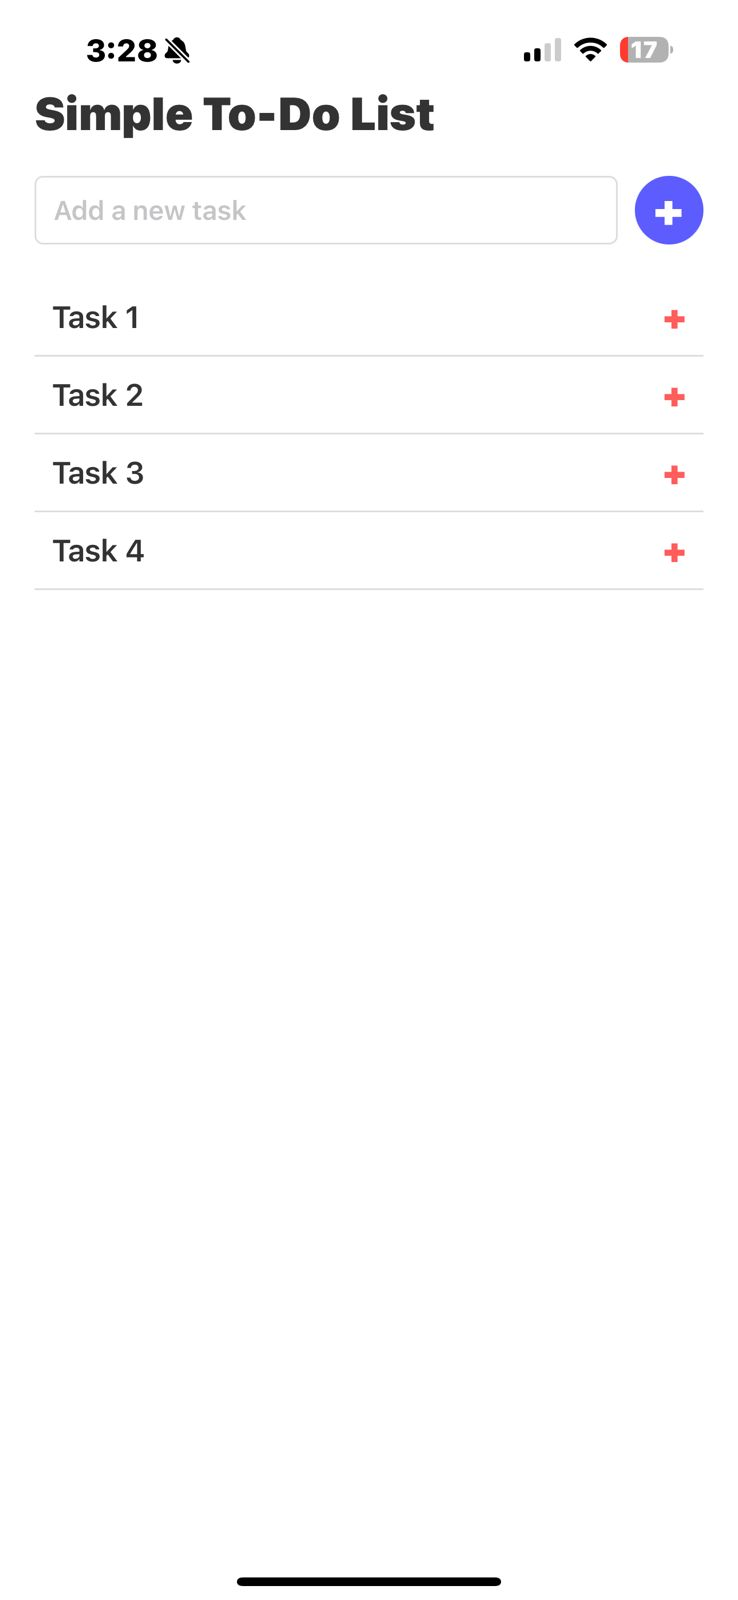
\includegraphics[width=0.5\textwidth]{AddTask.jpeg}
        \caption{Adding Task}
    \end{figure}

    \item \textbf{Update Existing Tasks:} Users can modify tasks they have already created.
    \begin{figure}[H]
        \centering
        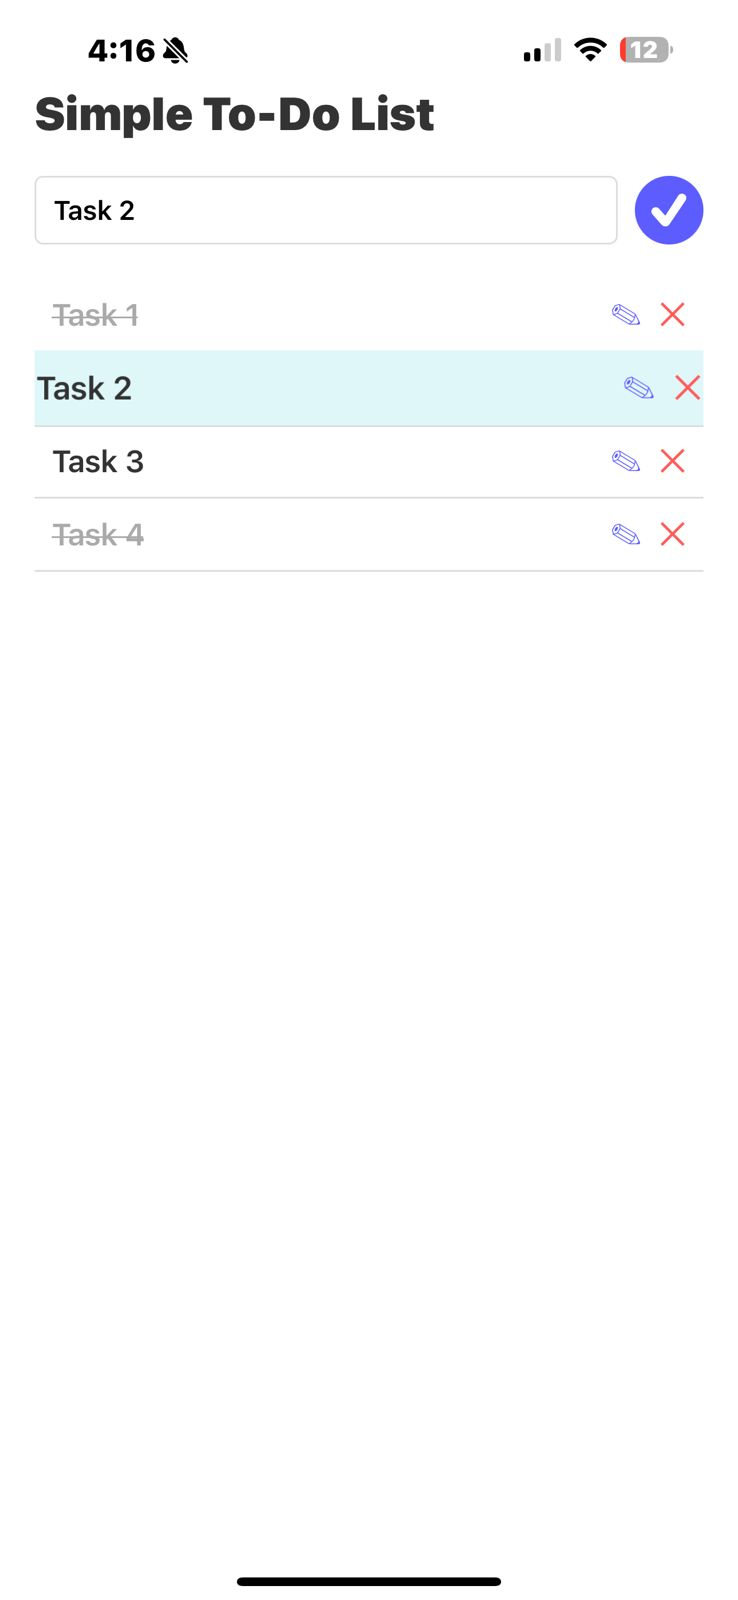
\includegraphics[width=0.5\textwidth]{EditTask.jpeg}
        \caption{Editing Task}
    \end{figure}
    
    
    \item \textbf{Delete Tasks:} Users can remove tasks from the list.
    \begin{figure}[H]
        \centering
        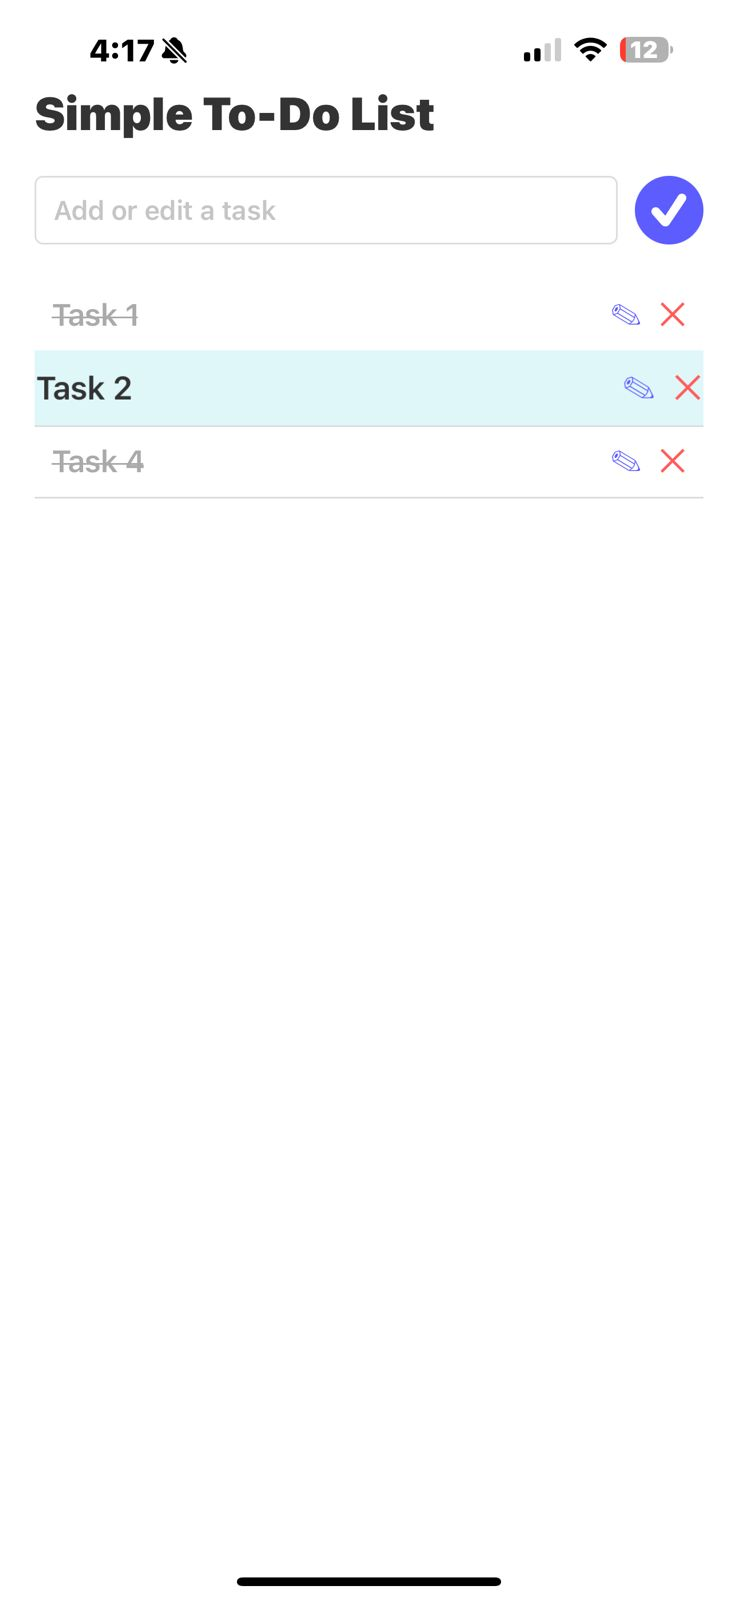
\includegraphics[width=0.5\textwidth]{DeleteTask.jpeg}
        \caption{Deleting Task}
    \end{figure}
  
    
    \item \textbf{Scrollable Task List:} The to-do list supports scrolling, allowing navigation through a large number of tasks.

    \item \textbf{User-Friendly Interface:} The app provides a simple and intuitive interface for managing tasks.
\end{itemize}

\subsection{Step 1: Set Up the Project}
\begin{enumerate}
    \item Create and navigate to the new project:
    \begin{verbatim}
    npx react-native init SimpleTodoApp
    cd SimpleTodoApp
    \end{verbatim}
    \begin{figure}[H]
        \centering
        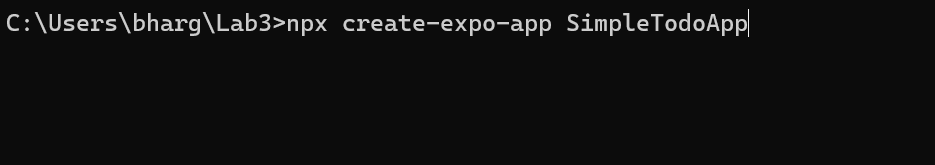
\includegraphics[width=0.5\textwidth]{SetUp.png}
        \caption{Setting up the To-Do List Project}
    \end{figure}
    
    \item Open the project in Visual Studio Code:
    \begin{verbatim}
    code .
    \end{verbatim}
\end{enumerate}

\subsection{Step 2: Create the Basic To-Do List Structure}
Replace the content of \texttt{App.js} with the following code:
\begin{figure}[H]
    \centering
    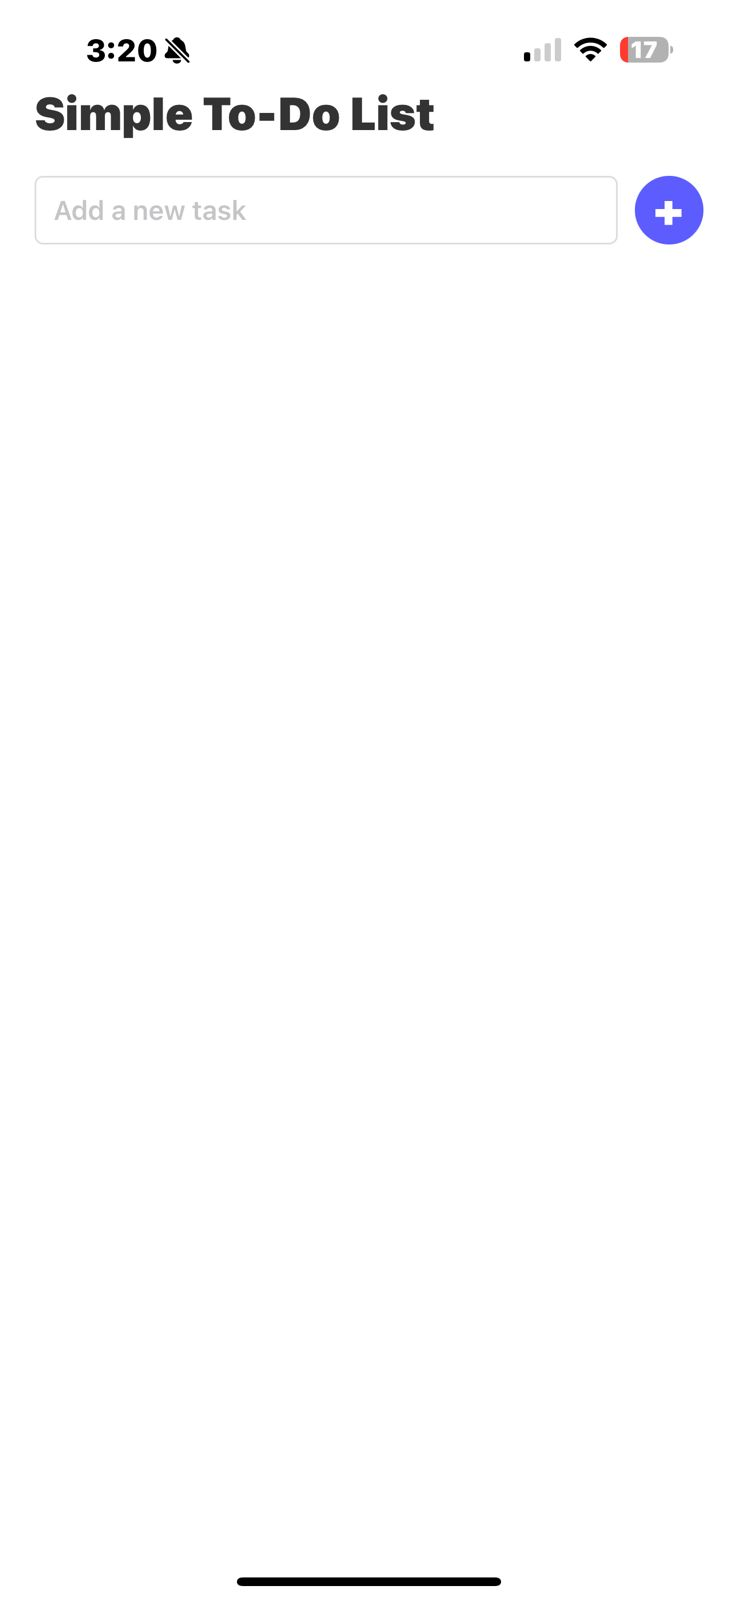
\includegraphics[width=0.5\textwidth]{InitialTodo.jpeg}
    \caption{Initial View of To-Do List}
\end{figure}


\subsection{Explanation of the Code}
\begin{itemize}
    \item \textbf{State Management}
    \begin{itemize}
        \item The \texttt{useState} hook is used to manage the state of the input field (task) and the list of tasks (tasks).
        \item When a new task is added, it updates the tasks array, and the input field is cleared.
    \end{itemize}
    
    \item \textbf{Adding a Task}
    \begin{itemize}
        \item The \texttt{addTask} function checks if the input is not empty.
        \item It adds a new task with a unique ID (using the current timestamp) to the tasks array.
        \item The input field is then reset to an empty string.
    \end{itemize}
    
    \item \textbf{Deleting a Task}
    \begin{itemize}
        \item The \texttt{deleteTask} function filters out the task with the specified ID from the tasks array.
        \item This updates the state and re-renders the list without the deleted task.
    \end{itemize}
    
    \item \textbf{Rendering the List}
    \begin{itemize}
        \item The \texttt{FlatList} component efficiently renders the list of tasks.
        \item Each item in the list displays the task text and a delete button.
    \end{itemize}
\end{itemize}

\subsection{Step 4: Running the App}
\begin{enumerate}
    \item In your terminal, run:
    \begin{verbatim}
    npx react-native run-android
    \end{verbatim}
    or
    \begin{verbatim}
    npx react-native run-ios
    \end{verbatim}
    \item This compiles and runs your app on the selected platform.
    \begin{figure}[H]
        \centering
        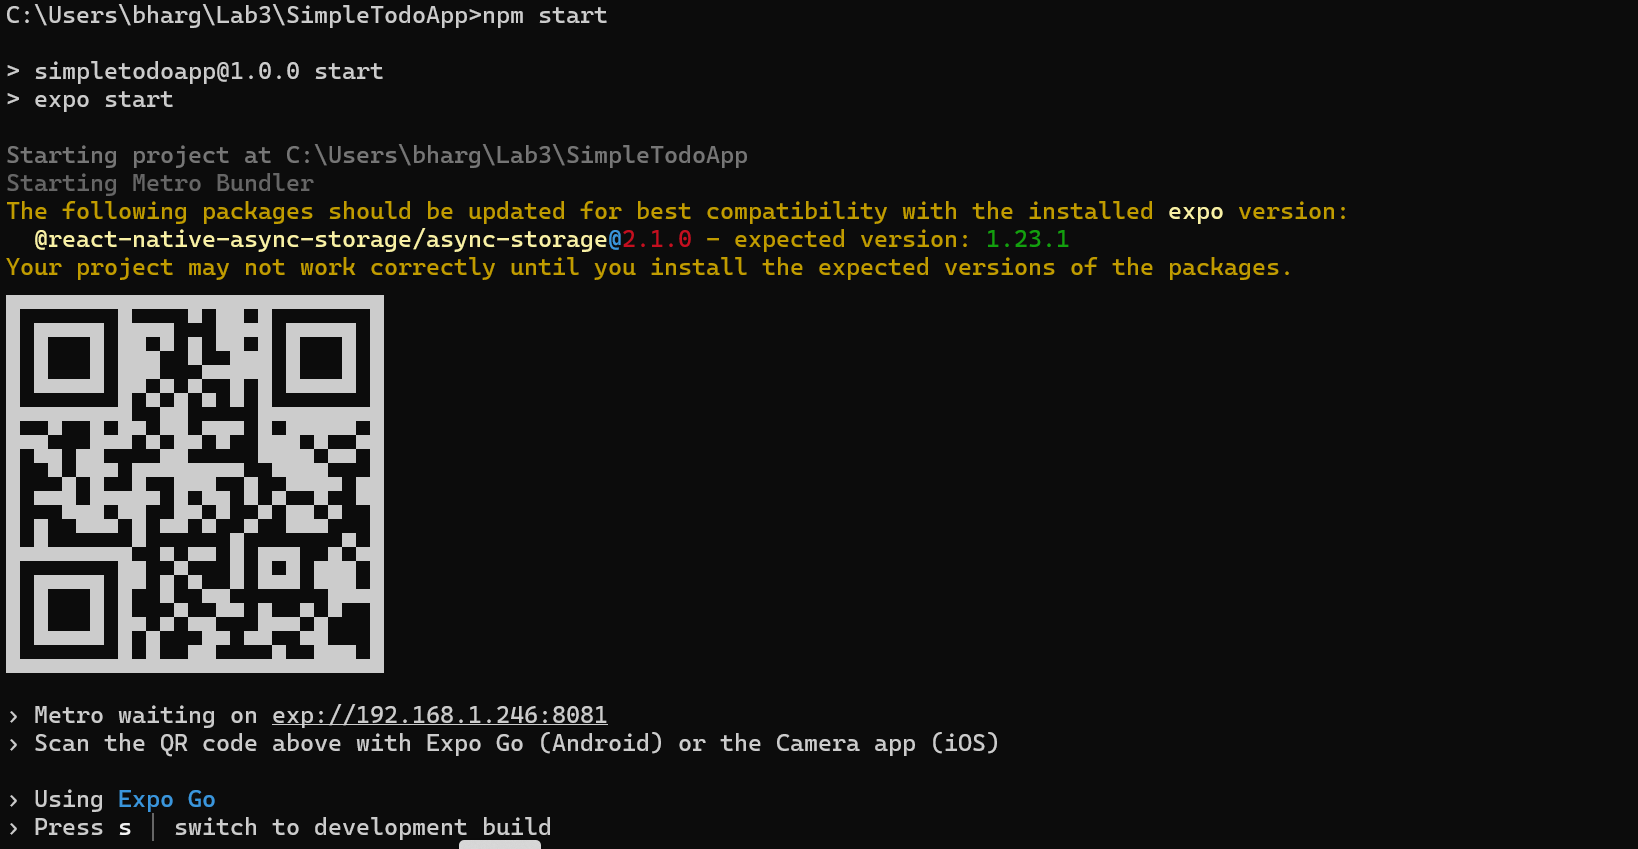
\includegraphics[width=0.5\textwidth]{RunningTodo.png}
        \caption{Running the To-Do List}
    \end{figure}

\end{enumerate}

\subsection{Submission (Total 60 Points)}
Provide detailed answers to the following questions, including any necessary screenshots:

\textbf{Extending Functionality (60 Points)}
\begin{itemize}
    \item \textbf{Mark Tasks as Complete (15 Points)}
    \begin{itemize}
        \item Add a toggle function that allows users to mark tasks as completed.
        \item Style completed tasks differently, such as displaying strikethrough text or changing the text color.
        \begin{figure}[H]
            \centering
            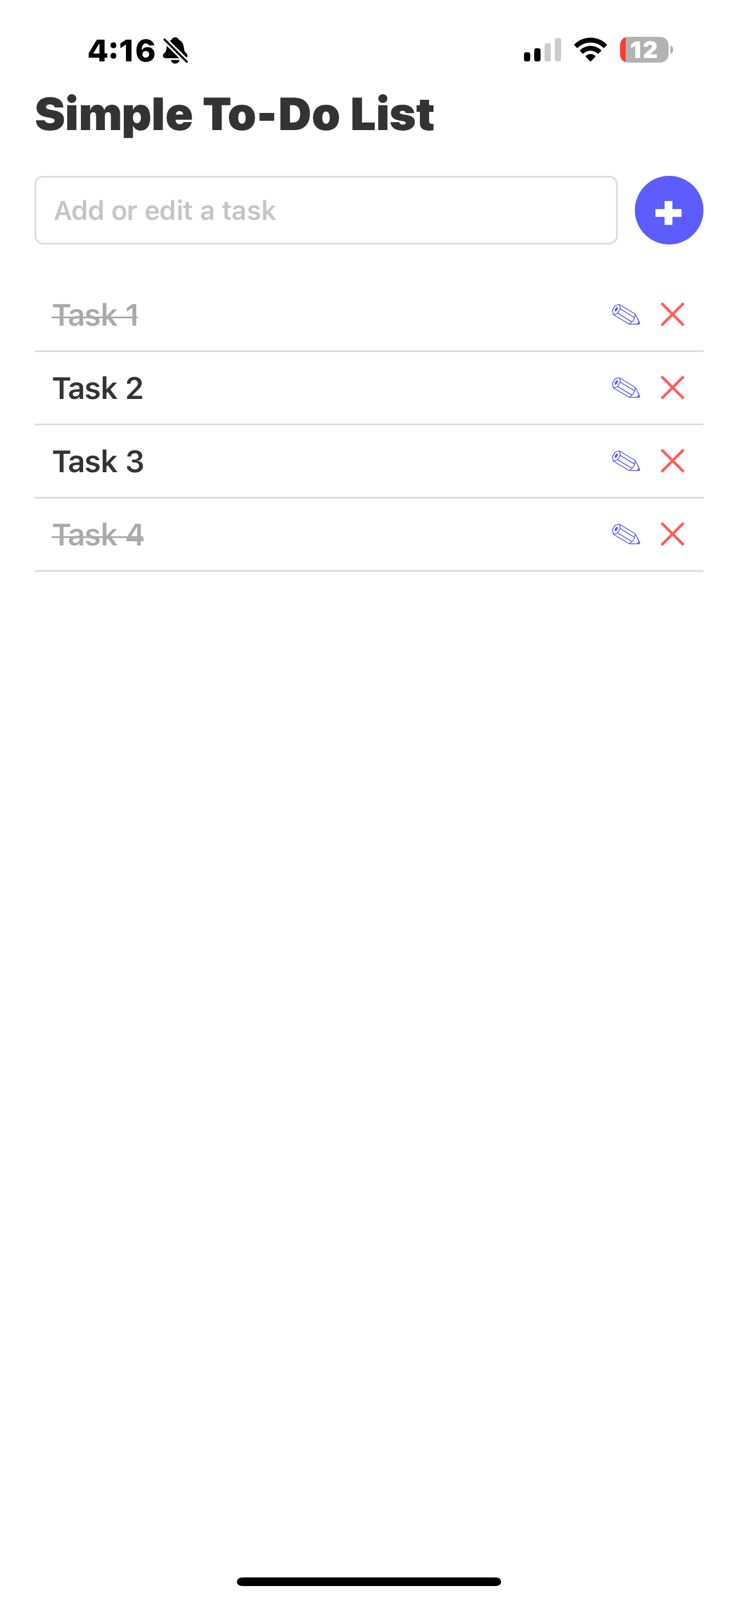
\includegraphics[width=0.5\textwidth]{MarkTask.jpeg}
            \caption{Task Marked as Complete}
        \end{figure}
     
        \item Explain how you updated the state to reflect the completion status of tasks.
        \item To update the state and reflect the completion status of tasks, a new property `isCompleted` was added to each task object in the `tasks` array, which tracks whether a task is marked as completed. The `toggleTaskCompletion` function was implemented to toggle this property by creating a new array where only the targeted task's `isCompleted` value is updated. This new array is then set to the `tasks` state using `setTasks`, and the updated list is persisted to AsyncStorage for data retention. To visually differentiate completed tasks, a conditional style was applied, adding a strikethrough and changing the text color to gray if `isCompleted` is true. React's state management automatically re-renders the `FlatList` with these changes, providing immediate feedback to the user.
    \end{itemize}
    
    \item \textbf{Persist Data Using AsyncStorage (15 Points)}
    \begin{itemize}
        \item Implement data persistence so that tasks are saved even after the app is closed.
        \item Use AsyncStorage to store and retrieve the tasks list.
        \begin{figure}[H]
            \centering
            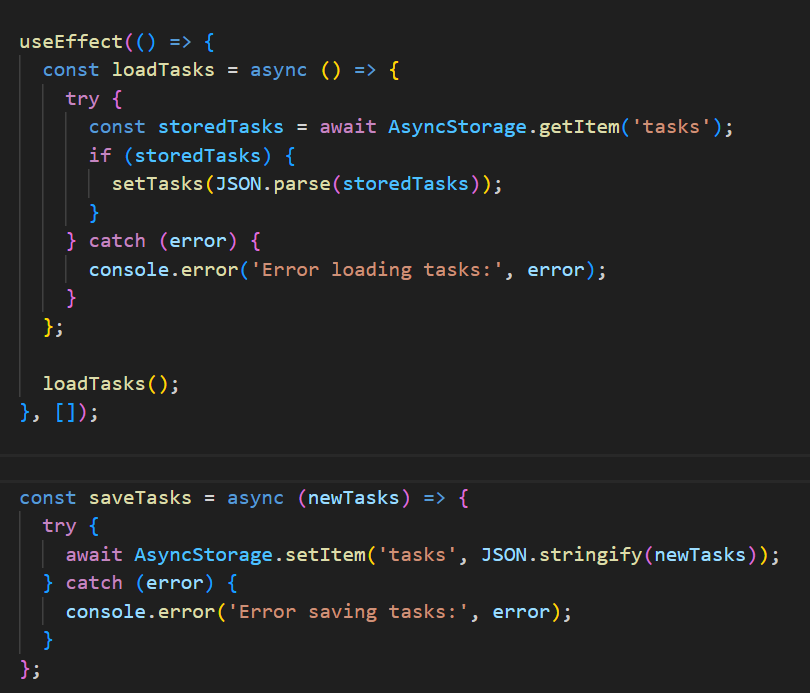
\includegraphics[width=0.5\textwidth]{Async.png}
            \caption{AsyncStorage Code Snippet}
        \end{figure}
    \end{itemize}
    
    \item \textbf{Edit Tasks (10 Points)}
    \begin{itemize}
        \item Allow users to tap on a task to edit its content.
        \item Implement an update function that modifies the task in the state array.
        \begin{figure}[H]
            \centering
            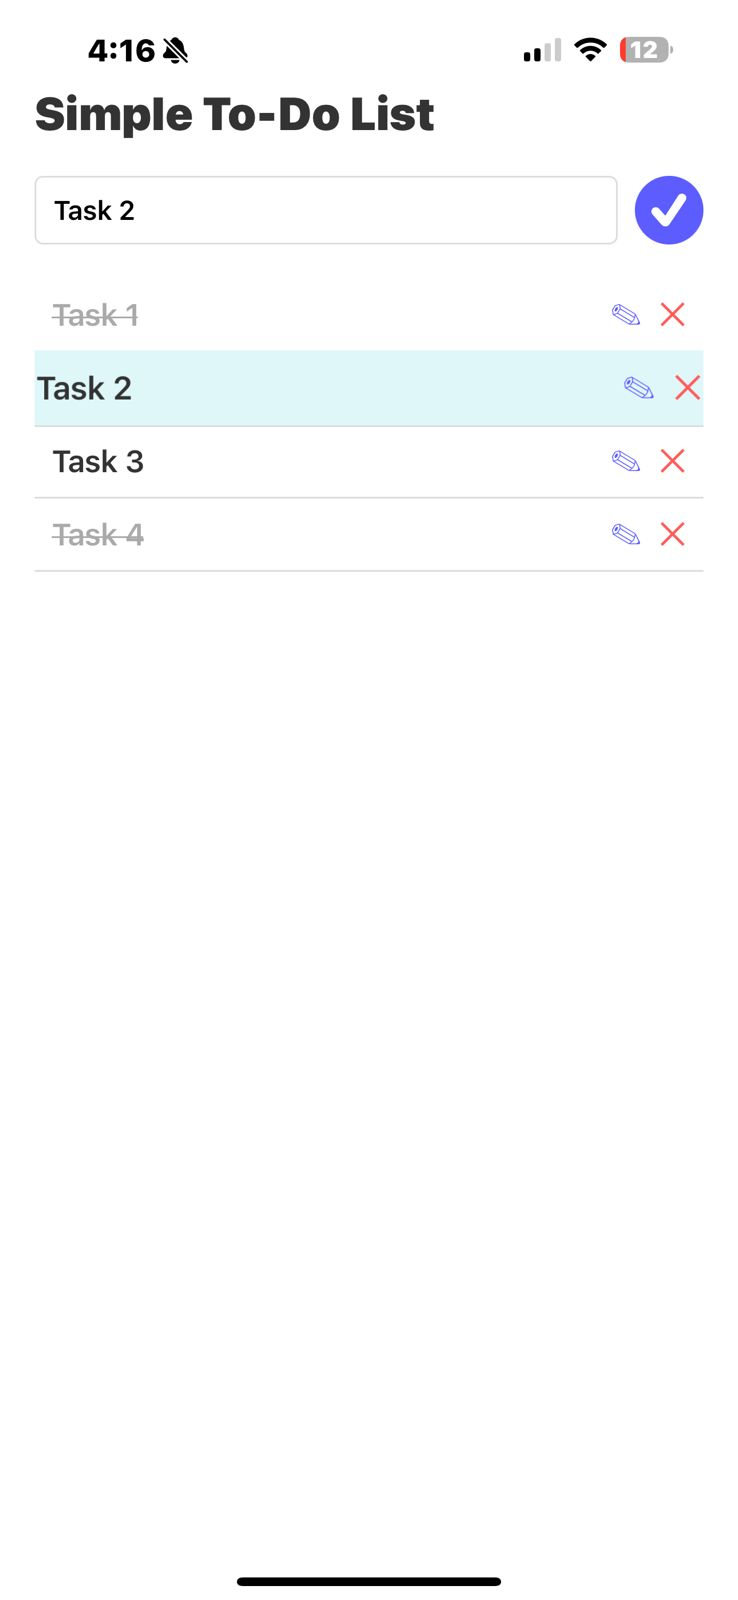
\includegraphics[width=0.5\textwidth]{EditTask.jpeg}
            \caption{Editing Task in the To-Do List}
        \end{figure}

        \item Explain how you managed the UI for editing tasks.
        \item To manage the UI for editing tasks, I implemented a system where tapping on a task allows users to modify its content. The task being edited is identified using the `editingTaskId` state, which stores the ID of the task currently being edited. When a task is selected for editing, its text is pre-filled into the input field, allowing users to make changes. The input field's value is controlled by the `task` state, which holds the current text being edited. Upon saving the changes, the `updateTask` function is called to update the task's text in the state by mapping over the `tasks` array and replacing the old text with the new one. The task list is then updated, and the changes are persisted to AsyncStorage. Additionally, the add button's text changes to a checkmark when editing, giving users a visual cue that the task is being edited. After updating, the input field is cleared, and `editingTaskId` is reset to `null` to signal the end of the editing process. This approach ensures a smooth and intuitive editing experience while maintaining state consistency.
    \end{itemize}
    
    \item \textbf{Add Animations (10 Points)}
    \begin{itemize}
        \item Use the \texttt{Animated} API from React Native to add visual effects when adding or deleting tasks.
        \item Describe the animations you implemented and how they enhance user experience.
             \item I implemented two key animations in the app using React Native's `Animated` API: fade-in and fade-out. When a task is added, it smoothly fades into view, enhancing the user experience by making the addition feel polished and dynamic. Similarly, when a task is deleted, it fades out before being removed, providing a smoother transition and visual feedback. These animations make the app feel more fluid and responsive, reducing abrupt changes and creating a more engaging interaction. Overall, they contribute to a polished user interface by providing clear and visually appealing feedback during task additions and deletions.
        \begin{figure}[H]
            \centering
            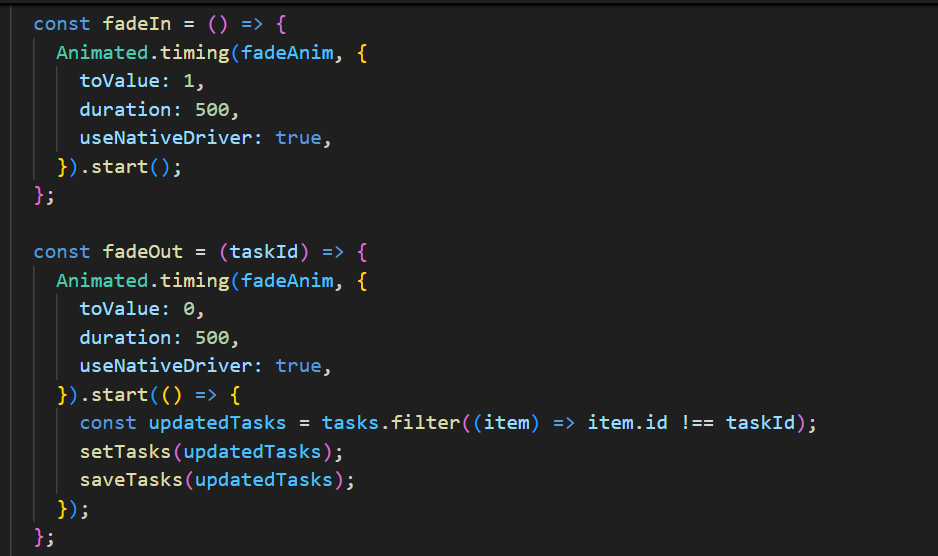
\includegraphics[width=0.5\textwidth]{Animation.png}
            \caption{Code Snippet for Adding Animations Using Animated API}
        \end{figure}
    \end{itemize}
\end{itemize}

\section{Conclusion}
This report provides an overview of setting up a development environment for React Native, configuring an emulator, comparing development options, and building a simple To-Do List app with extended functionality. The setup allows for efficient app development, testing, and deployment on both emulators and physical devices.

\section{Acknowledgment of LLM Assistance}
During the course of setting up the development environment and fixing certain errors, I utilized a Language Learning Model (LLM) for assistance. Specifically, the LLM provided solutions for resolving JAVA\_HOME path verification issues and offered advice on handling the default \texttt{App.tsx} compilation problem.

\end{document}
